% !TEX encoding = UTF-8
% !TEX TS-program = pdflatex
% !TEX root = ../arsclassica.tex
% !TEX spellcheck = it-IT

%************************************************
\chapter{Creazione di dataset relativi al traffico}
\label{cap:tsis-sensors}
%************************************************
Al fine di valutare le prestazioni degli algoritmi di apprendimento e classificazione delle \acl{CTBN} è emersa la necessità di generare dei dataset adeguati a tale scopo.

Come già specificato in precedenza, le \acs{CTBN} sono un modello stocastico dedito alla rappresentazione dell'evoluzione di sistemi dinamici, cioè di fenomeni cangianti nel tempo (non necessariamente o esclusivamente in base ad esso) rappresentabili come insiemi di traiettorie multi-variate. Si è quindi scelto di generare dei dataset che rappresentassero un tipico sistema cangiante: il traffico automobilistico su rete stradale.

Tali dataset, costituiti da un insieme di documenti rappresentanti la presenza (durante l'evolvere del tempo) di veicoli sui sensori di una rete stradale, sono stati generati con l'ausilio di un software commerciale, \acf{TSIS} (versione $\geq$ 6.2) e di una sua \acl{RTE} appositamente sviluppata al fine di monitorare e tracciare il passaggio dei veicoli. 

In questo capitolo si presentano sia i succitati strumenti utilizzati per la creazione di reti stradali e relativi modelli di simulazione, sia lo strumento creato per la creazione di dataset relativi al traffico.

Relativamente, invece, al processo pratico di creazione dei dataset si rimanda alla~\autoref{sec:create-dataset-howto}.

\section{TSIS}
\label{sec:tsis}
\acf{TSIS} è un \acl{IDE}\footnote{Un \acl{IDE}, comunemente chiamato anche \ACF{IDE}, è un insieme di programmi finalizzati a supportare il processo di sviluppo dei software. Generalmente, un \acs{IDE} è costituito da uno strumento per la creazione e modifica del codice sorgente, un compilatore o un interprete, strumenti per l'automazione dello sviluppo e la qualità del codice sorgente.}, distribuito commercialmente da McTrans\footnote{McTrans Moving Technology: \url{http://mctrans.ce.ufl.edu}} e supportato dalla \acf{FWHA}\footnote{Agenzia del Dipartimento dei Trasporti degli Stati Uniti d'America: \\ \url{www.fhwa.dot.gov}}, il cui scopo ultimo è permettere la simulazione e l'analisi di modelli di reti stradali.

\acs{TSIS} è costituito da insieme di strumenti dedicati alla creazione di reti stradali e relativi modelli di simulazione, all'esecuzione, e eventualmente alla visualizzazione, di tali modelli, così come all'interpretazione dei risultati ottenuti. Tale insieme di strumenti è reso accessibile tramite delle interfaccie grafiche\footnote{Un'interfaccia grafica, nota anche come \acf{GUI}, è un tipo di interfaccia utente il cui fine è permettere all'utente di interagire con il software manipolando oggetti grafici convenzionali.}.

L'architettura modulare con cui \acs{TSIS} è realizzato permette, in caso di necessità, di estendere tale ambiente creando degli ulteriori strumenti.

Di seguito si introducono brevemente i concetti relativi a \acs{TSIS} utilizzati nel prosieguo di questo lavoro di tesi.

Tuttavia si osservi che, poiché lo scopo di questo capitolo non consiste nel documentare \acs{TSIS}, la trattazione dei suoi dettagli tecnici (\eg{}, significato e lista dei tipi di dati rappresentabili) è omessa. A tale fine si rimanda invece alla documentazione ufficiale del software in questione.

\begin{definizione}[Progetto \acs{TSIS}]\label{defn:tsis-proj}
Un progetto \acs{TSIS} è un insieme di modelli di simulazione per una specifica rete stradale.
\end{definizione}

\begin{definizione}[Modello di simulazione \acs{TSIS}]\label{defn:tsis-sim-model}
Un modello di simulazione è costituito da un input (\eg{}, variazioni dei flussi di ingresso nella rete, variazioni delle percentuali di svolta dei veicoli nelle intersezioni) per la simulazione di una determinata rete stradale e tutti i dati generati dalla sua esecuzione (\ie{}, simulazione).
\end{definizione}
\begin{osservazione}
Un modello di simulazione può anche prevedere che la sua esecuzione sia eseguita più volte. Finché il seme dei numeri casuali non è modificato, esso è sempre considerato un singolo modello di simulazione.
\end{osservazione}

\begin{definizione}[Formato \acs{TRF}]\label{defn:trf-format}
\acs{TRF}\footnote{\acf{TRF}} è il formato dei file accettati dal simulatore di \acs{TSIS}. Esso codifica e rappresenta una rete stradale specificandone i vari componenti tramite l'utilizzo dei rispettivi \acs{RT}\footnote{\acf{RT}}, cioè delle righe di testo contenenti un codice identificativo numerico e i valori per i rispettivi campi accettati nell'ordine prestabilito. Allo stesso modo, tale formato incorpora il modello di simulazione della rete stradale che descrive.
\end{definizione}
\begin{osservazione}
Il formato \acs{TRF} è equivalente al formato \acs{TRAF}\footnote{\acf{TRAF}}.
\end{osservazione}

\begin{definizione}[Formato \acs{TNO}]\label{defn:tno-format}
\acs{TNO}\footnote{\acf{TNO}} è il formato nativo con cui vengono rappresentate in memoria le reti stradali create visivamente tramite l'interfaccia grafica \acs{TRAFED}.
\end{definizione}

\subsection{Caratteristiche}
% TODO: panoramica features (se si trova una lista già fatta solo da inserire)
% TODO: spiegare per grandi linee come funziona TSIS/CORSIM (time periods, time intervals etc.)

\subsection{Componenti}

In questa sezione si elencano gli strumenti che costituiscono l'ambiente di sviluppo \acs{TSIS}.

\begin{description}
\item[CORSIM] \hfill \\
\acs{CORSIM}\footnote{\acf{CORSIM}} costituisce il componente principale dell'insieme di strumenti denominato \acs{TSIS}. È un simulatore il cui obiettivo è permettere la creazione e l'esecuzione di modelli di simulazione \acs{TSIS}. È composto da due simulatori integrati che rappresentano l'intero sistema di traffico come funzione del tempo: \acs{NETSIM}\footnote{\acf{NETSIM}} e \acs{FREESIM}\footnote{\acf{FREESIM}}. Tali simulatori integrati rappresentano, rispettivamente, il traffico sulle strade urbane e non. La simulazione effettuata da tali strumenti è di tipo microscopico: essi modellano individualmente il comportamento di ogni singolo veicolo, prendendo in considerazione per ognuno di essi una serie di variabili, anche di tipo stocastico (\eg{}, tipologia di guidatore). Per tale motivo \acs{CORSIM} è dotato di molte possibili opzioni di configurazione e permette lo studio di modelli molto complessi e dettagliati.
\item[TRAFED] \hfill \\
\acs{TRAFED}\footnote{\acf{TRAFED}} è una \acs{GUI} il cui scopo è permettere la creazione e la modifica di reti stradali e di modelli di simulazione per \acs{CORSIM}.
\item[TShell] \hfill \\
\acs{TShell}\footnote{\acf{TShell}} è la \acs{GUI} di \acs{TSIS}. Funge da contenitore degli strumenti (preconfigurati, o creati dall'utente) di questo ambiente di sviluppo integrato e permette la gestione dei progetti \acs{TSIS}.
\item[TRAFVU] \hfill \\
\acs{TRAFVU}\footnote{\acf{TRAFVU}} è una \acs{GUI} finalizzata alla visualizzazione dei modelli di simulazione simulati con \acs{CORSIM}. Essa permette sia di visualizzare in modo animato l'evoluzione del traffico nella rete stradale con una qualsiasi granularità temporale, sia di visualizzare una serie di misure di interesse relative alla simulazione.
\item[TSIS Text Editor] \hfill \\
\acs{TSIS} Text Editor è uno strumento il cui scopo è facilitare la modifica manuale dei file \acs{TRF}. A tale scopo esso visualizza per ogni \acs{RT} che si intende modificare sia la sua descrizione sia l'insieme dei campi supportati.
\item[TSIS Script Tool] \hfill \\
\acs{TSIS} Script Tool è uno strumento per la creazione, la modifica e l'esecuzione di codice \acs{VBS}\footnote{\acf{VBS}}. Questo strumento fornisce un meccanismo utile ad automatizzare le funzionalità di simulazione di \acs{TSIS} (\eg{}, esecuzioni multiple dello stesso modello di simulazione variando il seme dei numeri casuali che governa la distribuzione di ingresso dei veicoli nella rete stradale).
\item[TSIS Translator] \hfill \\
\acs{TSIS} Translator è uno strumento utile alla conversione dei file dal formato \acs{TRF} al formato \acs{TNO} e viceversa. Tale operazione risulta utile al fine di rendere i file \acs{TRF} utilizzabili tramite lo strumento \acs{TRAFED} così come per rendere i file \acs{TNO} utilizzabili con \acs{CORSIM}.
\item[TSIS Output Processor] \hfill \\
\acs{TSIS} Output Processor è uno strumento finalizzato alla raccolta e l'aggregazione dei dati da \acs{CORSIM} durante l'esecuzione multipla di modelli di simulazione. La sua caratteristica principale consiste nella computazione automatica di un insieme di statistiche predefinite. Esso permette di scegliere sia le statistiche di interesse sia la granularità temporale della loro computazione.
\item[CORSIM RTE] \hfill \\
\acs{TSIS} fornisce un meccanismo finalizzato all'estensione delle sue funzionalità tramite la creazione, da parte dell'utente, di altri strumenti da integrare nell'ambiente di sviluppo. Queste estensioni, dette \acs{CORSIM} \acs{RTE}\footnote{\acf{RTE}}, possono interfacciarsi direttamente con \acs{CORSIM}, modificando o aumentando una parte della logica di simulazione, collezionando dati o monitorando eventi speciali.
\end{description}

\subsection{Estendere TSIS}
% panoramica sviluppo RTE
% TODO: descrizione delle varie API fornite da TSIS
% spostare ultima definizione CORSIM RTE qui? si dai ..
% in questa sezione presentaimo il funzionamento dell'interfacciamento tra CORSIM e strumenti esterni (CORSIM RTE) più dettagliatamente perché ci interessano al fine di ...
% presentiamo le API fornite dall'ambiente di sviluppo di TSIS
% mettere immagine di pulsante sensors in TSIS? far vedere come si aggiunge una RTE all'ambiente di TSIS (piccola sezione)

The FHWA's Traffic Software Integrated System (TSIS) is an integrated development environment that enables
users to conduct traffic operations analysis. Built using component architecture, TSIS is a toolbox that contains
tools that allow the user to define and manage traffic analysis projects, define traffic networks and create inputs for
traffic simulation analysis, execute traffic simulation models, and interpret the results of those models.
Although TSIS comes pre-configured with a set of tools, the component architecture is open and users can add their
own tools to the TSIS environment. Additionally, a user can provide extensions to the CORSIM simulation (part of
the TSIS package) using the run-time extension (RTE) interface described in this document. Run-time extensions
can be built to replace existing logic in CORSIM or to supplement its logic.

TSIS provides a mechanism by which an external application can interface directly with the CORSIM simulation
tool. This type of application has become known as a CORSIM run-time extension (RTE). The original run-time
extensions were tailored for signal timing studies. However, the concept has been expanded to support freeway
monitoring, incident detection, ramp metering and signal preemption.
The RTE capability enables CORSIM to operate with actual hardware in the loop. Some examples of these
hardware-in-the-loop experiments include using 170, NEMA, and 2070 controllers to control the signal states at
certain intersections in the simulation. In these experiments, the controller is interfaced to the simulation using a
Controller Interface Device (CID) that connects to the serial interface of the computer that hosts the simulation.
Another experiment involved using an advanced camera sensor and image processing software to estimate the queue
state of simulated vehicles as they approach an intersection. The queue states for the approaches to the intersection
are used by an adaptive control algorithm to make intelligent decisions about what the optimal signal state should
be. Run-time extensions can also be used to test adaptive signal control algorithms for effectiveness before they are
implemented in the field. With the rapid evolution of technology, these types of experiments are necessary, not only
to assess the benefits of advanced ITS applications, but to verify their operational capability before field
deployment.
This document describes how to construct a run-time extension and how to interface it with CORSIM and the TSIS
graphical user interface, known as TShell. It also describes in detail each of the interfaces that TSIS provides to
support RTE operation. Finally, the document presents a sample RTE.

\subsubsection{CORSIM}
The following figure illustrates the operation of CORSIM within the TSIS 6 architecture including the interfaces
that support the operation of run-time extensions. In the figure, the block arrows represent Component Object
Model (COM) interfaces and the thin arrows represent standard dynamic-link library (DLL) interfaces. In this
model, the CORSIM Driver Component is the TSIS tool that runs the CORSIM simulation and interfaces to the
TShell user interface. This component enables the user to control CORSIM execution and output processing, and
manages all user-supplied RTEs. Although the entire CORSIM architecture is shown for completeness, this
document will concentrate on describing the RTE interfaces marked 1, 2, 3, and 4 in the diagram.

\begin{figure}
\centering
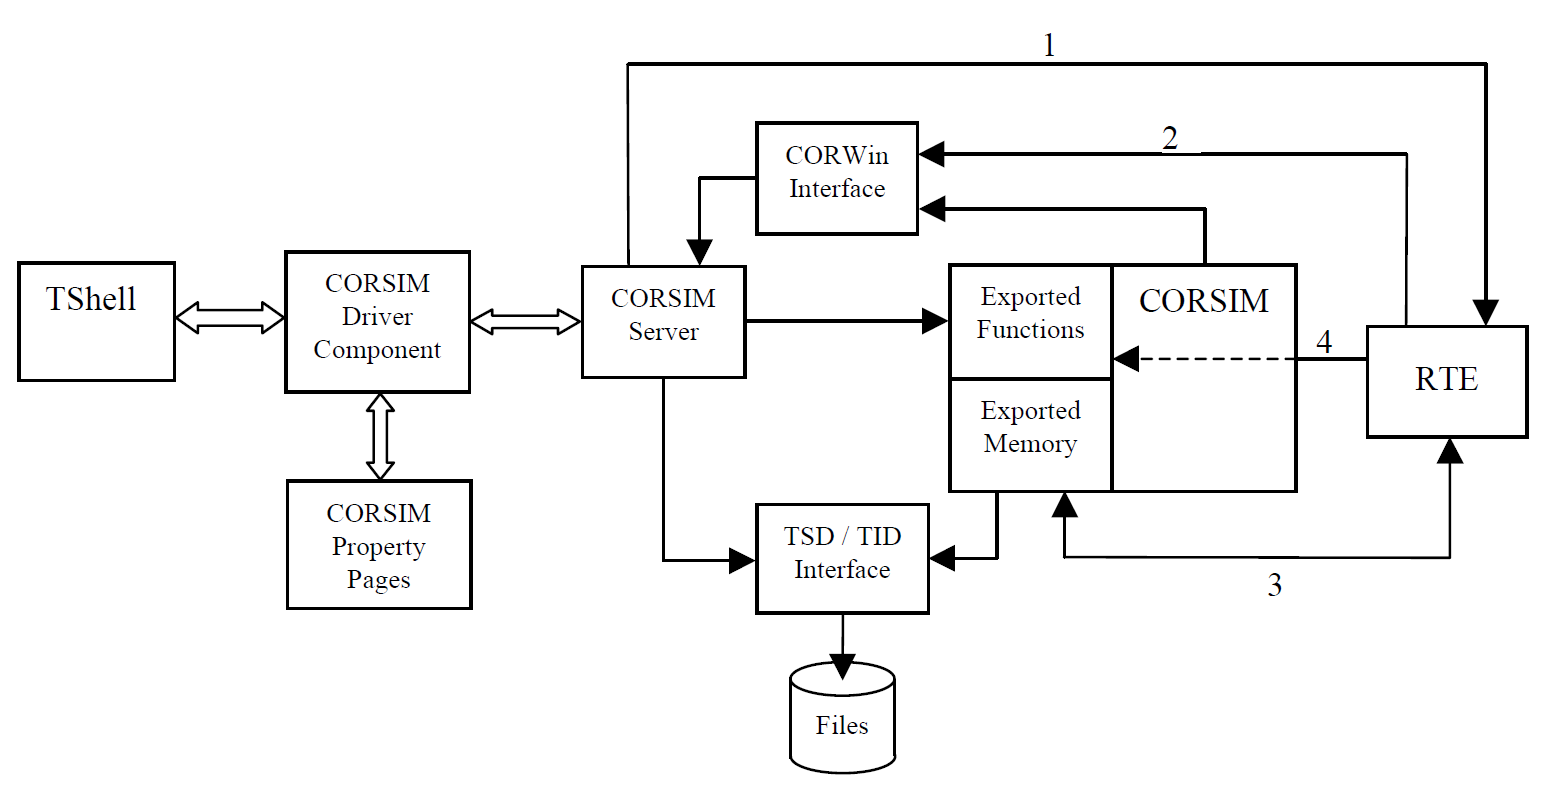
\includegraphics[width=1\columnwidth]{tsis-corsim-architecture}
\caption[L'architettura di \acs{CORSIM}]{Architettura modulare.}
\label{fig:tsis-corsim-arch}
\end{figure}


\subsubsection{CORWIN}

\subsubsection{CORSIM API}

\section{Estensione}
% TODO: introduzione, problema che deve risolvere

\subsection{Analisi}
% TODO: analisi del problema e del software che si è realizzato

\subsection{Sensors DLL}
% TODO: presentazione della DLL, progetto del software?

\section{Applicativi di supporto}
% TODO: discussione sulle operazioni utili alla creazione di dataset: insieme di file, ognuno dei quali è un insieme di traiettorie multivariate
